%\documentclass[a4paper]{article}
%\usepackage{geometry}
%\geometry{a4paper,scale=0.8}
\documentclass[8pt]{article}
\usepackage{ctex}
\usepackage{indentfirst}
\usepackage{longtable}
\usepackage{multirow}
\usepackage[a4paper, total={6.5in, 9in}]{geometry}
\usepackage{CJK}
\usepackage[fleqn]{amsmath}
\usepackage{parskip}
\usepackage{listings}
\usepackage{fancyhdr}

\pagestyle{fancy}

% 设置页眉
\fancyhead[L]{2024年秋季}
\fancyhead[C]{机器学习}
\fancyhead[R]{作业四}


\usepackage{graphicx}
\usepackage{float}
\usepackage{multicol}
\usepackage{amssymb}
\usepackage{booktabs}
\usepackage{xcolor}

% 定义Python代码风格
\definecolor{codegreen}{rgb}{0,0.6,0}
\definecolor{codegray}{rgb}{0.5,0.5,0.5}
\definecolor{codepurple}{rgb}{0.58,0,0.82}
\definecolor{backcolour}{rgb}{0.95,0.95,0.92}

\lstdefinestyle{mystyle}{
    backgroundcolor=\color{backcolour},   
    commentstyle=\color{codegreen},
    keywordstyle=\color{magenta},
    numberstyle=\tiny\color{codegray},
    stringstyle=\color{codepurple},
    basicstyle=\ttfamily\footnotesize,
    breakatwhitespace=false,         
    breaklines=true,     
    captionpos=b,        
    keepspaces=true,     
    numbers=left,        
    numbersep=5pt,       
    showspaces=false,    showstringspaces=false,
    showtabs=false,      
    tabsize=2
}

\lstset{style=mystyle}
\begin{document}

\textbf{\color{blue} \Large 姓名:毛九弢 \ \ \ 学号:221900175 \ \ \ \today}


\section*{一. (30 points) 随机森林的原理}

集成学习是一种通用技术,通过将多个不同模型的预测结果结合起来,以平均值或多数投票的方式生成单一预测,从而有效应对过拟合问题。


1. 考虑一组互不相关的随机变量 $\{Y_i\}_{i=1}^n$,其均值为 $\mu$,方差为 $\sigma^2$。  
请计算这些随机变量平均值的期望和方差,给出计算过程。  
提示:在集成方法的背景下,这些 $Y_i$ 类似于分类器 $i$ 所作的预测。(5 points)

\textbf{\large 解:}

设 $Y_i$ 的平均值为 $\bar{Y} = \frac{1}{n} \sum_{i=1}^n Y_i$。

(1) 期望:根据期望线性性质,有:
\[
E(\bar{Y}) = E\left(\frac{1}{n} \sum_{i=1}^n Y_i\right) = \frac{1}{n} \sum_{i=1}^n E(Y_i) = \frac{1}{n} \sum_{i=1}^n \mu = \mu
\]

(2) 方差:

由于 $Y_i$ 互不相关,各协方差为0,即,和的方差等于各自方差之和。

所以有:
\[
\operatorname{Var}(\bar{Y}) = \operatorname{Var}\left(\frac{1}{n} \sum_{i=1}^n Y_i\right) = \frac{1}{n^2} \sum_{i=1}^n \operatorname{Var}(Y_i) = \frac{1}{n^2} \sum_{i=1}^n \sigma^2 = \frac{\sigma^2}{n}
\]

因此,这些随机变量平均值的期望为 $\mu$,方差为 $\frac{\sigma^2}{n}$。

\vspace{3em}

2. 在第1小问中,我们看到对于不相关的分类器,取平均可以有效减少方差。  
尽管现实中的预测不可能完全不相关,但降低决策树之间的相关性通常能减少最终方差。  
现在,重新考虑一组具有相关性的随机变量 $\{Z_i\}_{i=1}^n$,其均值为 $\mu$,方差为 $\sigma^2$,每个 $Z_i \in \mathbb{R}$ 为标量。  
假设对任意 $i \neq j$,$\operatorname{Corr}(Z_i, Z_j) = \rho$。  
提示:如果你不记得相关性与协方差之间的关系,请回顾你的概率论等课程内容。 
\begin{itemize}
\item
请计算随机变量 $Z_i$ 平均值的方差,以 $\sigma$、$\rho$ 和 $n$ 为变量表示,给出计算过程。(5 points)  
\item
当 $n$ 非常大时,会发生什么?这对于取平均的潜在有效性说明了什么?  
(……如果 $\rho$ 很大($| \rho | \approx 1$)会怎样?……如果 $\rho$ 非常小($|\rho| \approx 0$)又会怎样?……如果 $\rho$ 处于中等水平($|\rho| \approx 0.5$)呢?)  
无需严格推导——基于你得出的方差公式,用定性分析进行讨论即可。 (6 points)
\end{itemize}

\textbf{\large 解:}
\[
    \operatorname{Var}\left(\sum_{i=1}^{n}X_i\right)
=
\sum_{i=1}^{n}\operatorname{Var}\left(X_i\right)
+
2\sum_{i=1}^{n-1}\sum_{j=i+1}^{n}\operatorname{Cov}\left(X_i,X_j\right)
\]

(1) 随机变量 $Z_i$ 平均值的方差
\begin{align*}
& \operatorname{Var}(\bar{Z}) 
= \operatorname{Var}\left(\frac{1}{n} \sum_{i=1}^n Z_i\right) 
\\ & = \frac{1}{n^2} 
    \left(
    \sum_{i=1}^n \operatorname{Var}(Z_i)
    +
    2 \sum_{i=1}^{n-1} \sum_{j=i+1}^n \operatorname{Cov}(Z_i, Z_j)
    \right) 
= \frac{1}{n^2} 
    \left(
        \sum_{i=1}^n \operatorname{Var}(Z_i)
        +
        2 \sum_{i=1}^{n-1} \sum_{j=i+1}^n \operatorname{Corr}(Z_i, Z_j)\sigma^2
    \right) 
\\ &= \frac{1}{n^2} 
    \left(
        \sum_{i=1}^n \sigma^2 
        +
        2 \sum_{i=1}^{n-1} \sum_{j=i+1}^n \rho\sigma^2 
    \right)
= \frac{1 + (n-1)\rho}{n}\sigma^2
\end{align*}

(2)  当 $n$ 非常大时,这些随机变量$Z_i$平均值的方差会趋于 $\rho\sigma^2$。

(2.1) 如果 $\rho$ 很大($| \rho | \approx 1$), 那么方差会趋于 $\sigma^2$,即据平均值后,方差的期望与原先相比没有减小,说明取平均的有效性不明显。

(2.2) 如果 $\rho$ 非常小($|\rho| \approx 0$), 那么方差会趋于 $\sigma^2/n$,当 $n$ 非常大时,这个数趋于0,即据平均值后,方差的期望会大大减小,说明取平均的有效性明显。
    
(2.3) 如果 $\rho$ 处于中等水平($|\rho| \approx 0.5$)呢, 那么当 $n$ 非常大时,方差会趋于 $\frac{1}{2}\sigma^2$,即据平均值后,方差的期望会减小,说明取平均的有一定有效性。

但不管 $\rho$ 多大,取平均后的方差期望都不会比原先来得大,因此,概率上来看,取平均的有效性是有的,且$\rho$越小,取平均的有效性越好。

\vspace{3em}

3. Bagging 是一种通过随机化从同一数据集生成多个不同学习器的方法。给定一个大小为 $n$ 的训练集,Bagging 会通过有放回抽样生成 $T$ 个随机子样本集,每个子样本集大小为 $n'$。
在每个子样本集中,一些数据点可能会被多次选中,而另一些可能完全未被选中。
当 $n' = n$ 时,大约 $63\%$ 的数据点会被选中,而剩下的 $37\%$ 被称为袋外样本点(Out-of-Bag,OOB)。
\begin{itemize}
\item
为什么是 $63\%$?
提示:当 $n$ 很大时,某个样本点未被选中的概率是多少?请只考虑在任意一个子样本集中(而不是所有 $T$ 个子样本集)未被选中的概率。(7 points)
\item
关于决策树的数量 $T$。
集成中的决策树数量通常需要在运行时间和降低方差之间进行权衡(典型值范围从几十到几千棵树)。
而子样本大小 $n'$ 对运行时间的影响较小,因此选择 $n'$ 时主要考虑如何获得最优预测结果。
虽然常见实践是设置 $n' = n$,但这并非总是最佳选择。
你会如何建议我们选择超参数 $n'$? (7 points)
\end{itemize}

\textbf{\large 解:}

(1) 为什么是 $63\%$?

在$n'$次采样中,由于$n' = n$,所以一个样本从未被选中的概率是 $(1 - \frac{1}{n})^{n'} = (1 - \frac{1}{n})^{n}$,当 $n$ 很大时,这个概率趋于 $e^{-1} \approx 0.37$。
因此,在$n'$次采样中,一个样本被选中的概率趋于 $1 - 0.37 = 0.63$。

引入$I(x_i)$,表示在$n'$次采样中样本 $x_i$ 被选中的指示函数,那么 $E(I(x_i)) = 0.63$。
那么,被选中的不同的样本数的期望为$
E\left(\sum_{i=1}^{n}I(x_i)\right) 
= \sum_{i=1}^{n}E(I(x_i)) = 0.63n$。

那么,被选中的样本数占总样本数的比例为 $0.63$,即$63\%$。

(2) 关于决策树的数量 $T$ (超参数$n'$的选择)。

1. 数据集的大小:如果数据集较大,可以选择较大的 $n'$,以确保每个子样本集包含足够的信息。如果数据集较小,可以选择较小的 $n'$,以增加子样本集的多样性。

2. 模型的复杂度:如果模型较复杂,可以选择较大的 $n'$,以确保每个子样本集包含足够的信息。如果模型较简单,可以选择较小的 $n'$,以增加子样本集的多样性。

3. 交叉验证:可以通过交叉验证来选择最优的 $n'$,以确保模型的泛化能力。

总之,选择 $n'$ 时需要综合考虑数据集的大小、模型的复杂度和交叉验证的结果,以获得最优的预测结果。

\vspace{3em}

% \begin{lstlisting}[language=Python, caption=SMOTE模型接口]
% """
% 注意:
% 1. 这个框架提供了基本的结构,您需要完成所有标记为 'pass' 的函数。
% 2. 记得处理数值稳定性问题,例如在计算对数时避免除以零。
% 3. 在报告中详细讨论您的观察结果和任何有趣的发现。
% """
% class SMOTE(object):
%     def __init__(self , X, y, N, K, random_state =0):
%         self.N = N # 每个小类样本合成样本个数
%         self.K = K # 近邻个数
%         self.label = y # 进行数据增强的类别
%         self.sample = X
%         self.n_sample , self.n = self.sample.shape # 获得样本个数, 特征个数
    
%     def over_sampling(self):
%         pass
% \end{lstlisting}

% 4. 请说明SMOTE算法的缺点并讨论可能的改进方案(5 points)。




\section*{二. (20 points) 随机森林的实现}

在本题中,你将实现决策树和随机森林,用于在以下两个数据集上进行分类:1)垃圾邮件数据集,2)泰坦尼克号数据集(用于预测这场著名灾难的幸存者)。数据已随作业提供。

为方便起见,我们提供了初始代码,其中包括预处理步骤和部分功能的实现。你可以自由选择使用或不使用这些代码来完成实现。

\begin{lstlisting}[language=Python, caption=随机森林模型接口]
"""
注意:
1. 这个框架提供了基本的结构,您需要完成所有标记为 'pass' 的函数。
2. 记得处理数值稳定性问题,例如在计算对数时避免除以零。
3. 在报告中详细讨论您的观察结果和任何有趣的发现。
"""
from collections import Counter

import numpy as np
from numpy import genfromtxt
import scipy.io
from scipy import stats
from sklearn.tree import DecisionTreeClassifier, export_graphviz
from sklearn.base import BaseEstimator, ClassifierMixin
from sklearn.model_selection import cross_val_score
import pandas as pd
from pydot import graph_from_dot_data
import io

import random
random.seed(246810)
np.random.seed(246810)

eps = 1e-5  # a small number

class BaggedTrees(BaseEstimator, ClassifierMixin):

    def __init__(self, params=None, n=200):
        if params is None:
            params = {}
        self.params = params
        self.n = n
        self.decision_trees = [
            DecisionTreeClassifier(random_state=i, **self.params)
            for i in range(self.n)
        ]

    def fit(self, X, y):
        # TODO
        pass

    def predict(self, X):
        # TODO
        pass


class RandomForest(BaggedTrees):

    def __init__(self, params=None, n=200, m=1):
        if params is None:
            params = {}
        params['max_features'] = m
        self.m = m
        super().__init__(params=params, n=n)


class BoostedRandomForest(RandomForest):
    # OPTIONAL
    def fit(self, X, y):
        # TODO
        pass
    
    def predict(self, X):
        # TODO
        pass


def preprocess(data, fill_mode=True, min_freq=10, onehot_cols=[]):
    # Temporarily assign -1 to missing data
    data[data == b''] = '-1'

    # Hash the columns (used for handling strings)
    onehot_encoding = []
    onehot_features = []
    for col in onehot_cols:
        counter = Counter(data[:, col])
        for term in counter.most_common():
            if term[0] == b'-1':
                continue
            if term[-1] <= min_freq:
                break
            onehot_features.append(term[0])
            onehot_encoding.append((data[:, col] == term[0]).astype(float))
        data[:, col] = '0'
    onehot_encoding = np.array(onehot_encoding).T
    data = np.hstack(
        [np.array(data, dtype=float),
         np.array(onehot_encoding)])

    # Replace missing data with the mode value. We use the mode instead of
    # the mean or median because this makes more sense for categorical
    # features such as gender or cabin type, which are not ordered.
    if fill_mode:
        # TODO
        pass

    return data, onehot_features


def evaluate(clf):
    print("Cross validation", cross_val_score(clf, X, y))
    if hasattr(clf, "decision_trees"):
        counter = Counter([t.tree_.feature[0] for t in clf.decision_trees])
        first_splits = [
            (features[term[0]], term[1]) for term in counter.most_common()
        ]
        print("First splits", first_splits)


if __name__ == "__main__":
    dataset = "titanic"
    # dataset = "spam"
    params = {
        "max_depth": 5,
        # "random_state": 6,
        "min_samples_leaf": 10,
    }
    N = 100

    if dataset == "titanic":
        # Load titanic data
        path_train = 'datasets/titanic/titanic_training.csv'
        data = genfromtxt(path_train, delimiter=',', dtype=None)
        path_test = 'datasets/titanic/titanic_testing_data.csv'
        test_data = genfromtxt(path_test, delimiter=',', dtype=None)
        y = data[1:, 0]  # label = survived
        class_names = ["Died", "Survived"]

        labeled_idx = np.where(y != b'')[0]
        y = np.array(y[labeled_idx], dtype=float).astype(int)
        print("\n\nPart (b): preprocessing the titanic dataset")
        X, onehot_features = preprocess(data[1:, 1:], onehot_cols=[1, 5, 7, 8])
        X = X[labeled_idx, :]
        Z, _ = preprocess(test_data[1:, :], onehot_cols=[1, 5, 7, 8])
        assert X.shape[1] == Z.shape[1]
        features = list(data[0, 1:]) + onehot_features

    elif dataset == "spam":
        features = [
            "pain", "private", "bank", "money", "drug", "spam", "prescription",
            "creative", "height", "featured", "differ", "width", "other",
            "energy", "business", "message", "volumes", "revision", "path",
            "meter", "memo", "planning", "pleased", "record", "out",
            "semicolon", "dollar", "sharp", "exclamation", "parenthesis",
            "square_bracket", "ampersand"
        ]
        assert len(features) == 32

        # Load spam data
        path_train = 'datasets/spam_data/spam_data.mat'
        data = scipy.io.loadmat(path_train)
        X = data['training_data']
        y = np.squeeze(data['training_labels'])
        Z = data['test_data']
        class_names = ["Ham", "Spam"]

    else:
        raise NotImplementedError("Dataset %s not handled" % dataset)

    print("Features", features)
    print("Train/test size", X.shape, Z.shape)

    # Decision Tree
    print("\n\nDecision Tree")
    dt = DecisionTreeClassifier(max_depth=3)
    dt.fit(X, y)

    # Visualize Decision Tree
    print("\n\nTree Structure")
    # Print using repr
    print(dt.__repr__())
    # Save tree to pdf
    graph_from_dot_data(dt.to_graphviz())[0].write_pdf("%s-basic-tree.pdf" % dataset)

    # Random Forest
    print("\n\nRandom Forest")
    rf = RandomForest(params, n=N, m=np.int_(np.sqrt(X.shape[1])))
    rf.fit(X, y)
    evaluate(rf)

    # Generate Test Predictions
    print("\n\nGenerate Test Predictions")
    pred = rf.predict(Z)

\end{lstlisting}

1. 请参考以上模板实现随机森林算法。你也可以选择不参考模板,自行实现,但是不允许使用任何现成的随机森林实现。不过你可以使用库中提供的单棵决策树实现(我们在模板代码中使用了sklearn.tree .DecisionTreeClassifier)。如果使用模板代码,你主要需要实现随机森林继承的超类,即bagged trees的实现,它会基于不同的数据样本创建并训练多棵决策树。完成后,请在模板中补充上缺失的部分。(5 points)

2.不需要长篇大论,每个问题用1-2句话回答即可:(5 points)
\begin{itemize}
\item 你是如何处理分类特征和缺失值的?
% \item 你实现的决策树的停止准则是什么?
\item 你是如何实现随机森林的?
\item 你是否采用了特殊的方法加速训练?(回答“没有”也是可以的。)
\item 还有什么特别棒的功能你实现了吗?(回答“没有”也是可以的。)
\end{itemize}

\textbf{\large 解:}

\vspace{3em}

3.对于这两个数据集,请分别训练一棵决策树和一个随机森林,并报告它们的训练准确率和测试准确率。  
你需要报告8个数字(2个数据集 $\times$ 2个分类器 $\times$ 训练/测试)。(5 points)

\textbf{\large 解:}

\vspace{3em}

4. 决策树和随机森林的决策分析。(5 points)
\begin{itemize}
\item
对于决策树,选择来自每个类别(垃圾邮件和正常邮件)的一条数据点,列出决策树为对其分类所做的分裂(即,在哪个特征上以及该特征的哪个值上进行分裂)。
以下是一个示例:

\begin{enumerate}
    \item (`hot") $\geq$ 2
    \item (`thanks") $<$ 1
    \item (`nigeria") $\geq$ 3
    \item 因此这封邮件是垃圾邮件。
\end{enumerate}

\begin{enumerate}
    \item (`budget") $\geq$ 2
    \item (`spreadsheet") $\geq$ 1
    \item 因此这封邮件是正常邮件。
\end{enumerate}

\item
对于随机森林,找出并列出树根节点处最常见的分裂。例如:

\begin{enumerate}
    \item (`viagra") $\geq$ 3 (20 trees)
    \item (`thanks") $<$ 4 (15 trees)
    \item (`nigeria") $\geq$ 1 (5 trees)
\end{enumerate}

\end{itemize}

\textbf{\large 解:}

\vspace{3em}


\section*{三. (20 points) 聚类理论}

聚类是一种无监督学习任务,其核心是根据数据样本之间的相似性(通常由距离度量定义)将数据分成若干个簇。常用聚类算法如 \( k \)-均值和 DBSCAN 都需要特定的距离度量和超参数设置。以下问题围绕距离度量、目标函数、以及超参数设置展开:  

1. 
在聚类算法中,距离度量是衡量样本间相似性的基础,选择合适的距离度量对聚类效果有显著影响(5 points)。  

(a) 给定样本 \( x = (x_1, x_2, \dots, x_d) \) 和 \( y = (y_1, y_2, \dots, y_d) \),分别写出以下三种常见距离度量的数学公式: 
\begin{itemize}
    \item 欧几里得距离  
    \item 曼哈顿距离
    \item 余弦相似度(将其转换为距离形式)  
\end{itemize}

(b) 在以下场景中,分析哪种距离更适合使用,并简要说明原因:  
\begin{itemize}
    \item 场景 1:高维稀疏特征向量(如文本数据的 TF-IDF 表示)   
    \item 场景 2:二维几何分布数据(如图像中的空间点分布)  
\end{itemize}

\textbf{\large 解:}

(1) 数学公式:
\begin{itemize}
    \item 欧几里得距离:\( d(x, y) = \sqrt{\sum_{i=1}^d (x_i - y_i)^2} \)
    \item 曼哈顿距离:\( d(x, y) = \sum_{i=1}^d |x_i - y_i| \)
    \item 余弦相似度:\( \text{sim}(x, y) = \frac{x \cdot y}{\|x\| \cdot \|y\|} = \frac{\sum_{i=1}^{d}{x_i y_i}}{
        \sqrt{\sum_{i=1}^{d}{x_i^2}} \sqrt{\sum_{i=1}^{d}{y_i^2}}
    } \) 
\end{itemize}

(2) 选择距离

\begin{itemize}
    \item 场景 1:高维稀疏特征向量(如文本数据的 TF-IDF 表示)

    余弦相似度更适合使用。原因是高维稀疏特征向量的绝对值大小可能差异很大,欧几里得距离和曼哈顿距离会受到向量长度的影响,而余弦相似度关注的是向量的方向,能够更好地衡量稀疏向量之间的相似性。其次,稀疏性使得余弦相似度的计算更加快捷高效。

    \item 场景 2:二维几何分布数据(如图像中的空间点分布)

    欧几里得距离更适合使用。原因是二维几何分布数据中的点的距离可以直接用欧几里得距离来衡量,欧几里得距离能够准确反映点与点之间的实际几何距离。
\end{itemize}
\vspace{3em}

2. \( k \)-均值聚类的目标函数与迭代过程, \( k \)-均值聚类的目标是最小化以下目标函数(10 points):  
\[
J = \sum_{i=1}^k \sum_{x \in C_i} \|x - \mu_i\|^2
\]  
其中,\( C_i \) 表示第 \( i \) 个聚类簇,\( \mu_i \) 为第 \( i \) 个簇的中心。  

(a) 推导在分配样本点到最近的簇中心时,为什么目标函数 \( J \) 会减少。 

(b) 推导为什么更新簇中心为簇内样本点的均值时,目标函数 \( J \) 会减少。 

(c) \( k \)-均值的超参数 \( k \) 对结果有何影响?  
\begin{itemize}
    \item  如果 \( k \) 设置过大或过小,分别可能会导致什么问题?  
    \item 提出一种确定 \( k \) 的方法,并解释其原理。  
\end{itemize}

\textbf{\large 解:}

(1) 推导在分配样本点到最近的簇中心时,为什么目标函数 \( J \) 会减少。

设样本点$x$, 原先的簇为$C_u$,更新后的簇为$C_v$,则有:
\[\|x-\mu_u\| \ge \|x-\mu_v\|\]

设进行这一个样本的分配前的目标函数值为$J_u$,分配后的目标函数值为$J_v$,则有:
\[J_v - J_u = - \|x-\mu_u\| + \|x-\mu_v\| \le 0 \]

也就是:分配样本点到最近的簇中心时,目标函数 \( J \) 会减少。

(2) 推导为什么更新簇中心为簇内样本点的均值时,目标函数 \( J \) 会减少。

(3) \( k \)-均值的超参数 \( k \) 对结果有何影响? 

\begin{itemize}
    \item 如果 \( k \) 设置过大
    \item 如果 \( k \) 设置过小  
\end{itemize}

一种确定 \( k \) 的方法:

原理如下:  

\vspace{3em}

3. 密度聚类(如 DBSCAN)依赖以下两个超参数(5 points):  
\begin{itemize}
    \item \( \varepsilon \)(邻域半径):定义一个点的邻域范围。  
    \item \( \text{MinPts} \)(核心点的最小邻域点数):定义核心点的密度阈值。 
\end{itemize}
(a) 核心点、边界点和噪声点的定义是什么?它们在聚类中的作用分别是什么?

(b) 如果 \( \varepsilon \) 和 \( \text{MinPts} \) 设置不当,可能会出现哪些问题?  
\begin{itemize}
    \item \( \varepsilon \) 过大或过小    
    \item \( \text{MinPts} \) 过大或过小  
\end{itemize}
   
(c) 为什么 DBSCAN 不需要预先指定聚类簇的数量 \( k \)?这对实际应用有什么优势?

\textbf{\large 解:}

\vspace{3em}

\section*{四. (30 points) 聚类实战}
使用商场客户数据集(Mall Customer Dataset)完成客户分群分析。该数据集包含客户的年龄(Age)、年收入(Annual Income)和消费积分(Spending Score)等特征。你需要通过实现和优化聚类算法来完成客户画像分析。数据随作业提供。

{\color{red}代码见Prob4文件夹中,使用了作业提供的初始代码。}

1. 在不借助外部实现的情况下,手动实现KMeans方法(4 points),在数据集上进行聚类,可视化聚类结果(3 points),并解决下列问题(3 points):
\begin{itemize}
    \item 如何使用肘部法则确定合适的k值,绘图说明
    \item 简单分析每个客户群的特征
    \item 计算和分析簇内平方和(inertia)
\end{itemize}


\textbf{\large 解:}

task1 中,我们固定了随机种子为14,以保证结果的可重复性。

1.0. Kmeans算法实现见{\color{blue}Prob4/kmeans.py中},K=5时,可视化聚类结果如下:

\begin{figure}[H]
    \centering
    \begin{minipage}{0.32\textwidth}
        \centering
        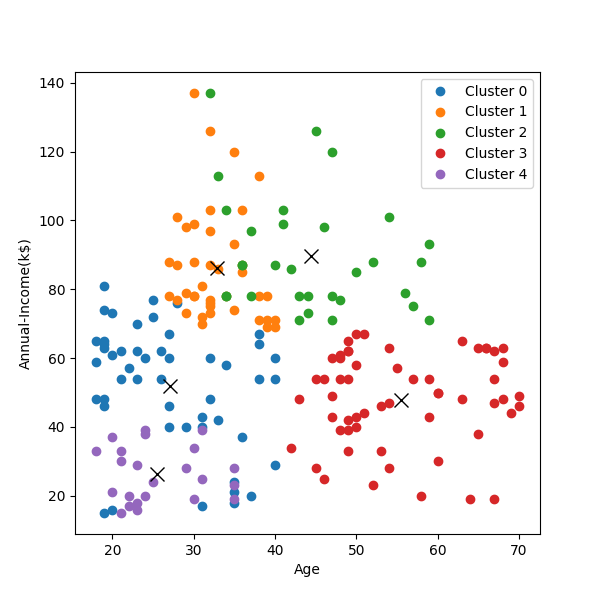
\includegraphics[width=\textwidth]{./Prob4/out/task1_rand14/images/cluster_result_k5_0_1.png}
        \caption{Age vs. Annual Income}
        \label{fig: Age vs. Annual Income k5}
    \end{minipage}
    \hfill
    \begin{minipage}{0.32\textwidth}
        \centering
        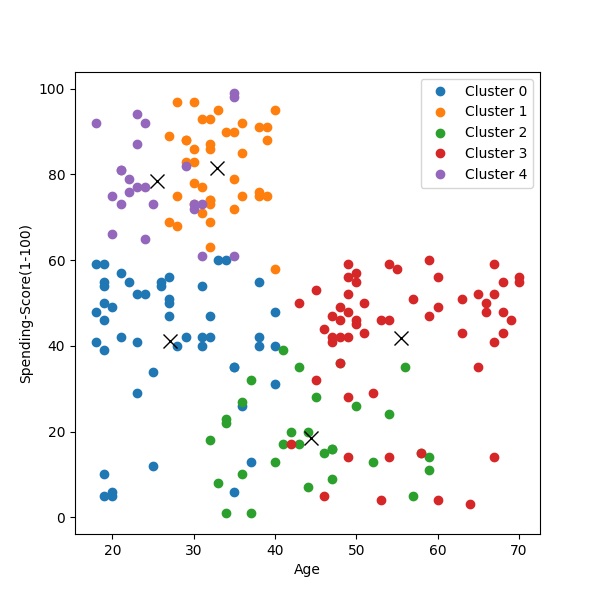
\includegraphics[width=\textwidth]{./Prob4/out/task1_rand14/images/cluster_result_k5_0_2.png}
        \caption{Age vs. Spending Score}
        \label{fig: Age vs. Spending Score k5 rand14}
    \end{minipage}
    \hfill
    \begin{minipage}{0.32\textwidth}
        \centering
        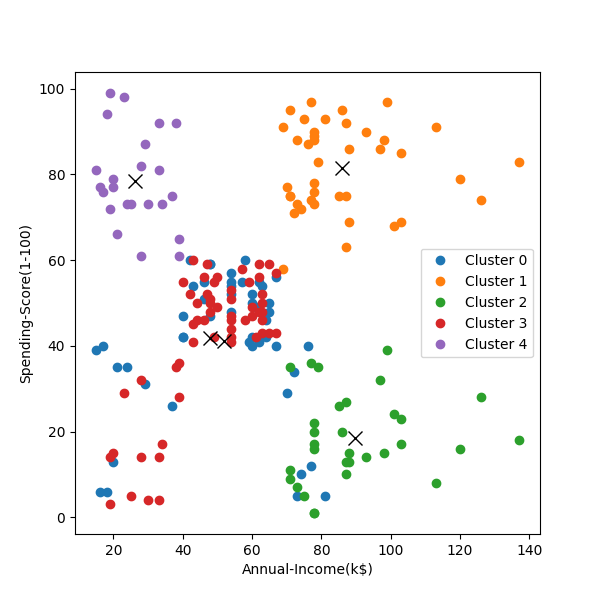
\includegraphics[width=\textwidth]{./Prob4/out/task1_rand14/images/cluster_result_k5_1_2.png}
        \caption{Annual Income vs. Spending Score}
        \label{fig: Annual Income vs. Spending Score k5 rand14}
    \end{minipage}
    \hfill
    \begin{minipage}{0.32\textwidth}
        \centering
        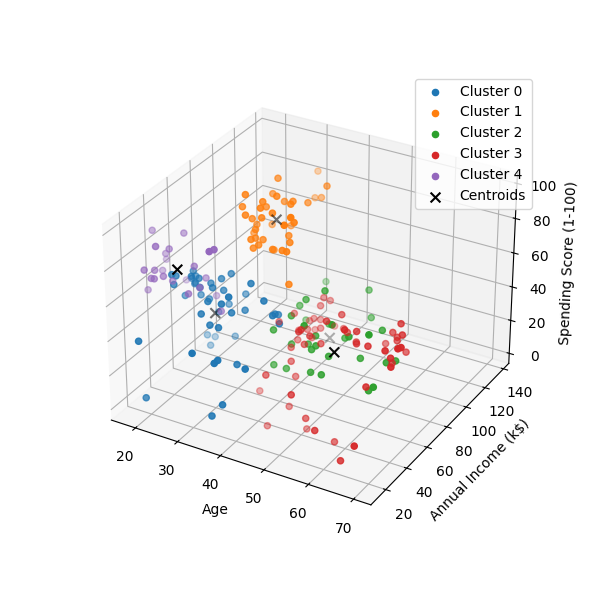
\includegraphics[width=\textwidth]{./Prob4/out/task1_rand14/images/cluster_result_k5_3d.png}
        \caption{3D Visualization}
        \label{fig: 3D Visualization k5 rand14}
    \end{minipage}
    \hfill
    \begin{minipage}{0.32\textwidth}
        \centering
        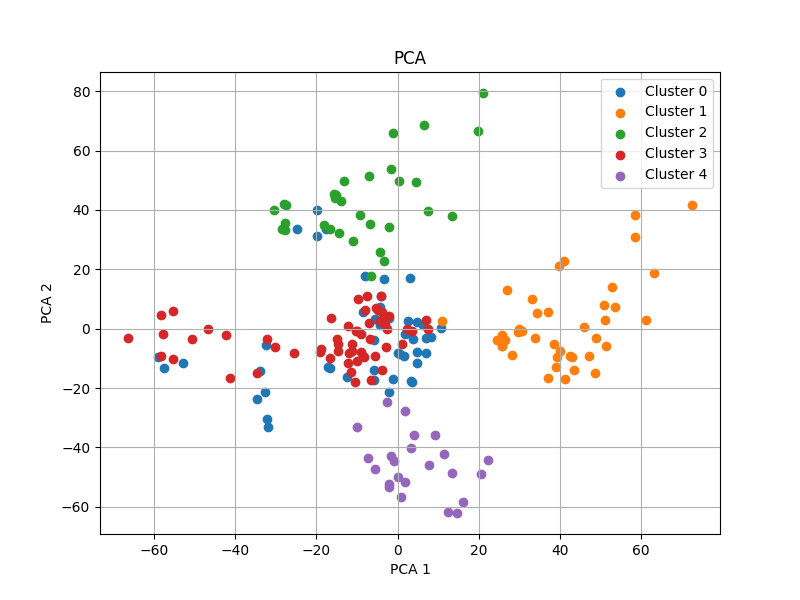
\includegraphics[width=\textwidth]{./Prob4/out/task1_rand14/images/PCA_k5.png}
        \caption{PCA Visualization}
        \label{fig: PCA Visualization k5 rand14}
    \end{minipage}
    \hfill
    \begin{minipage}{0.32\textwidth}
        \centering
        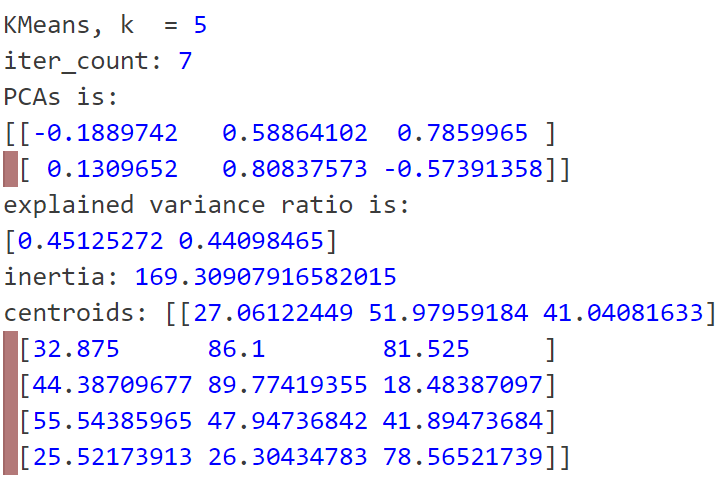
\includegraphics[width=\textwidth]{./Prob4/out/task1_rand14/log_k5.png}
        \caption{Log}
        \label{fig: log_k5.png rand14}
    \end{minipage}
\end{figure}

1.1. 簇内平方和 与 K值关系如下图所示:
\begin{figure}[H]
    \centering
    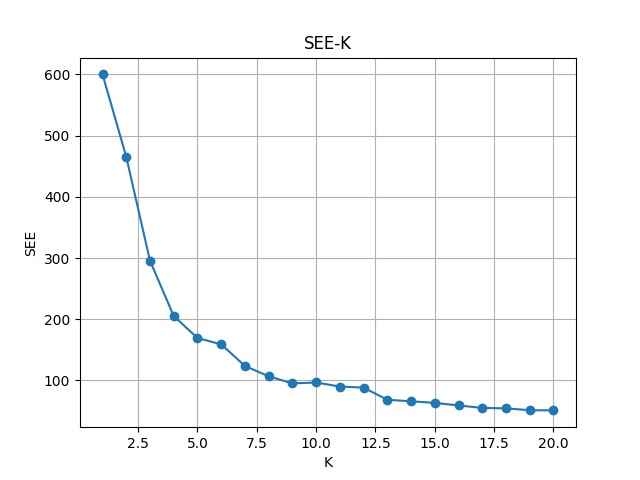
\includegraphics[width=0.5\textwidth]{./Prob4/out/task1_rand14/SEE-K.png}
    \caption{Inertia vs. K}
    \label{fig: Inertia vs. K rand14}
\end{figure}
肘部法则确定合适的k值,从图中可以看出,当K=5和7时,簇内平方和的下降速度变缓,因此选择K=5或者7。
之后我们进行了轮廓系数的计算,K=5时,轮廓系数为0.3898,稳定性0.6299;K=7时,轮廓系数为0.4223,稳定性0.7555。一定程度上说明K=7时的聚类效果更好。


K=5时,见图\ref{fig: Age vs. Spending Score k5 rand14}-图\ref{fig: log_k5.png rand14},K=7时,视图如下:
\begin{figure}[H]
    \centering
    \begin{minipage}{0.32\textwidth}
        \centering
        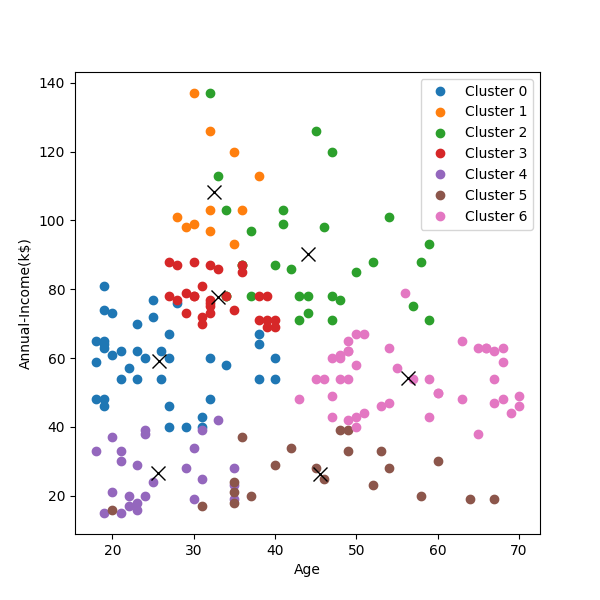
\includegraphics[width=\textwidth]{./Prob4/out/task1_rand14/images/cluster_result_k7_0_1.png}
        \caption{Age vs. Annual Income}
        \label{fig: Age vs. Annual Income k7}
    \end{minipage}
    \hfill
    \begin{minipage}{0.32\textwidth}
        \centering
        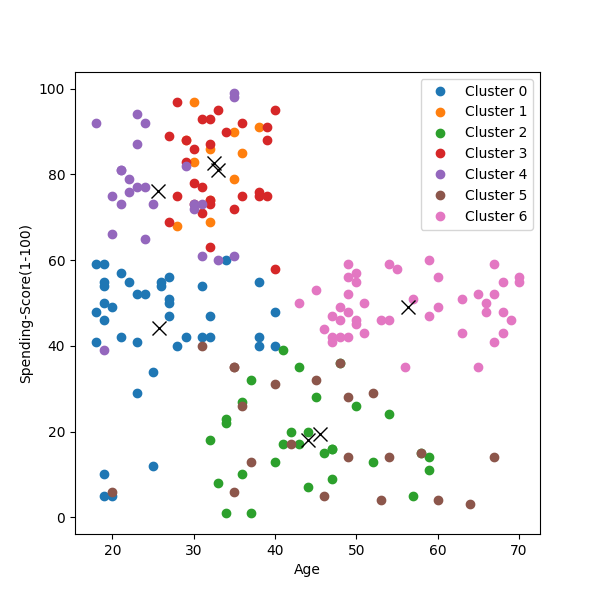
\includegraphics[width=\textwidth]{./Prob4/out/task1_rand14/images/cluster_result_k7_0_2.png}
        \caption{Age vs. Spending Score}
        \label{fig: Age vs. Spending Score k7 rand14}
    \end{minipage}
    \hfill
    \begin{minipage}{0.32\textwidth}
        \centering
        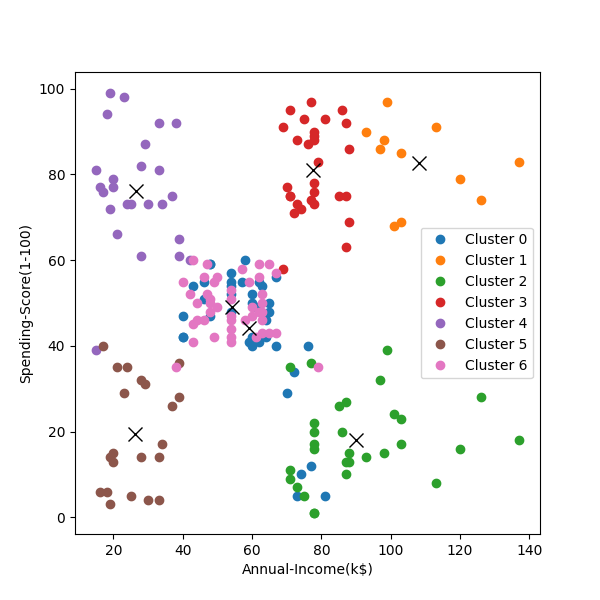
\includegraphics[width=\textwidth]{./Prob4/out/task1_rand14/images/cluster_result_k7_1_2.png}
        \caption{Annual Income vs. Spending Score}
        \label{fig: Annual Income vs. Spending Score k7 rand14}
    \end{minipage}
    \hfill
    \begin{minipage}{0.32\textwidth}
        \centering
        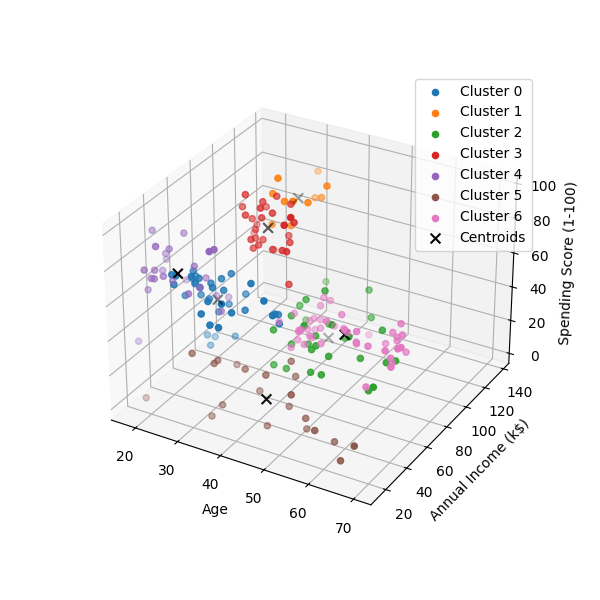
\includegraphics[width=\textwidth]{./Prob4/out/task1_rand14/images/cluster_result_k7_3d.png}
        \caption{3D Visualization}
        \label{fig: 3D Visualization k7 rand14}
    \end{minipage}
    \hfill
    \begin{minipage}{0.32\textwidth}
        \centering
        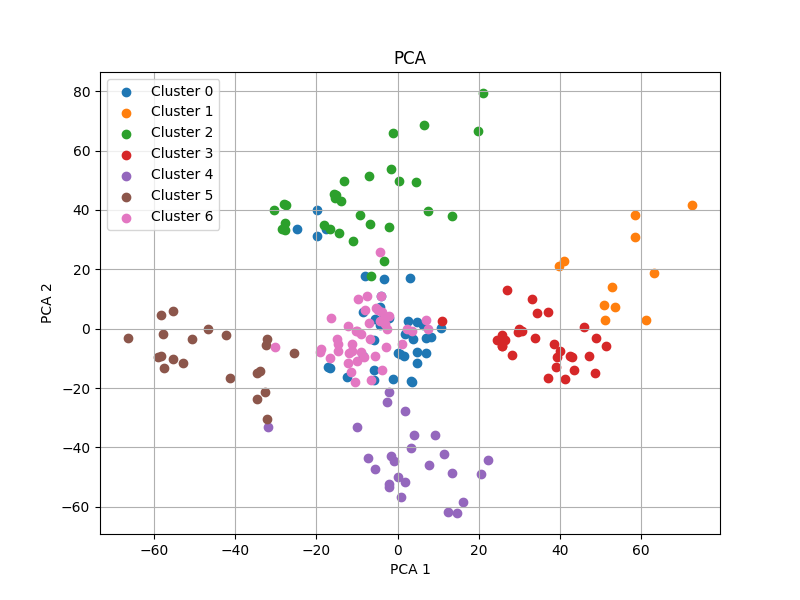
\includegraphics[width=\textwidth]{./Prob4/out/task1_rand14/images/PCA_k7.png}
        \caption{PCA Visualization}
        \label{fig: PCA Visualization k7 rand14}
    \end{minipage}
    \hfill
    \begin{minipage}{0.32\textwidth}
        \centering
        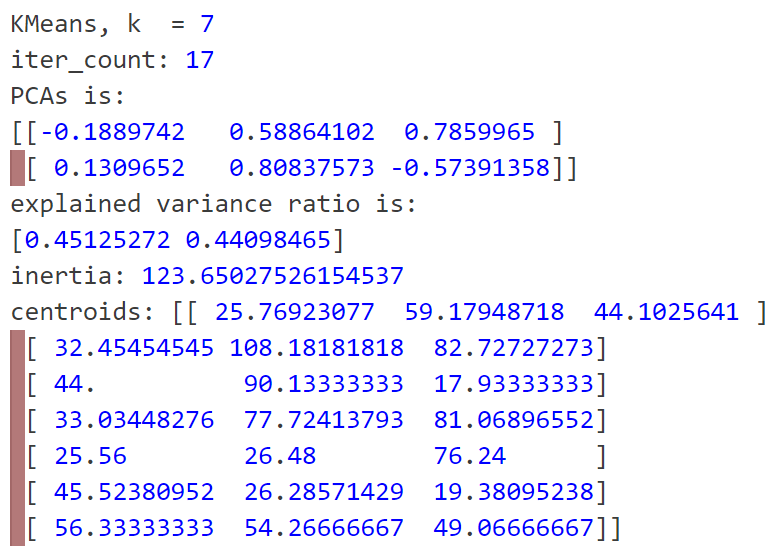
\includegraphics[width=\textwidth]{./Prob4/out/task1_rand14/log_k7.png}
        \caption{Log}
        \label{fig: log_k7.png rand14}
    \end{minipage}
\end{figure}

1.2. 简单分析每个客户群的特征 我们以 K=7 为例,对每个簇的特征进行分析:

\begin{itemize}
    \item Cluster 0: 青年到中青年;年收入中等偏下;消费积分中等,有部分消费积分较低的客户。
    \item Cluster 1: 中青年;年收入高;消费积分高;
    \item Cluster 2: 中年;年收入中等偏上,部分收入较高;消费积分较低,大部分较低。
    \item Cluster 3: 中青年;年收入中等,消费积分高。
    \item Cluster 4: 青年到中青年;年收入低,消费积分较高。
    \item Cluster 5: 几乎覆盖所有年龄段,青年较少;年收入低;消费积分较低。
    \item Cluster 6: 中老年;年收入中等偏下;消费积分中等。
\end{itemize}

1.3. 计算和分析簇内平方和(inertia) 见图\ref{fig: Inertia vs. K rand14},随着K值的增加,簇内平方和逐渐减小,但是减小速度逐渐变缓。

\vspace{3em}

2. 基于问题一的实现,我们发现随机初始化可能导致结果不稳定。请实现和分析以下改进:
\begin{itemize}
    \item 实现K-means++初始化方法(4分)
    \item 实现聚类评估指标(3分):轮廓系数(Silhouette Score)、聚类稳定性评估
    \item 对比分析(3分)
    \begin{enumerate}
        \item 比较随机初始化和K-means++的结果差异,可以通过可视化聚类图进行对比
\item 比较两种方法的稳定性
\item 分析初始化对收敛速度的影响
    \end{enumerate}
\end{itemize}

\textbf{\large 解:}

2.0. 实现K-means++初始化方法,代码见{\color{blue}./Prob4/kmeans\text{\_}pp.py中}

\begin{figure}[H]
    \centering
    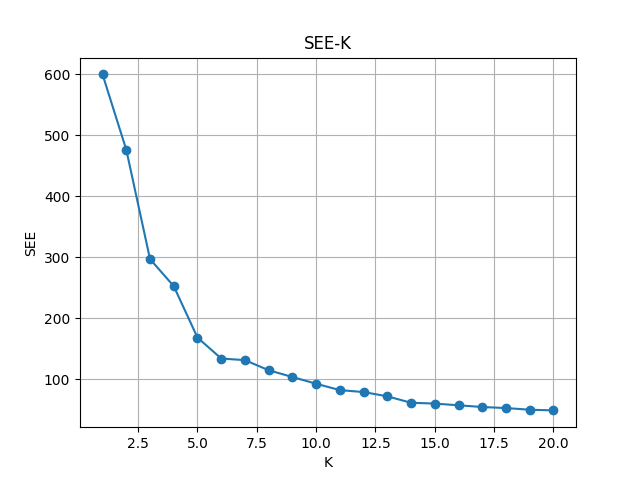
\includegraphics[width=0.5\textwidth]{./Prob4/out/task2_rand14/SEE-K.png}
    \caption{K-means++ 簇内平方和 与 K值关系}
    \label{fig: Inertia vs. K rand14 pp}
\end{figure}

根据 肘部法则,我们选取K=6,进行聚类,可视化聚类结果如下:

\begin{figure}[H]
    \centering
    \begin{minipage}{0.32\textwidth}
        \centering
        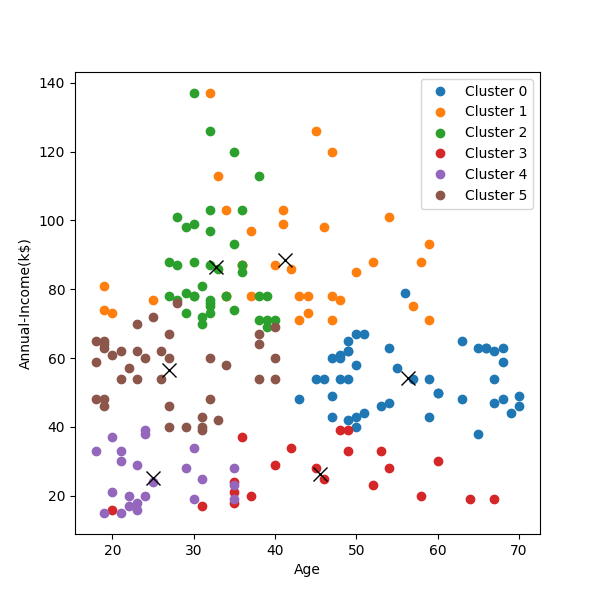
\includegraphics[width=\textwidth]{./Prob4/out/task2_rand14/images/cluster_result_k6_0_1.png}
        \caption{Age vs. Annual Income}
        \label{fig: Age vs. Annual Income k6 pp}
    \end{minipage}
    \hfill
    \begin{minipage}{0.32\textwidth}
        \centering
        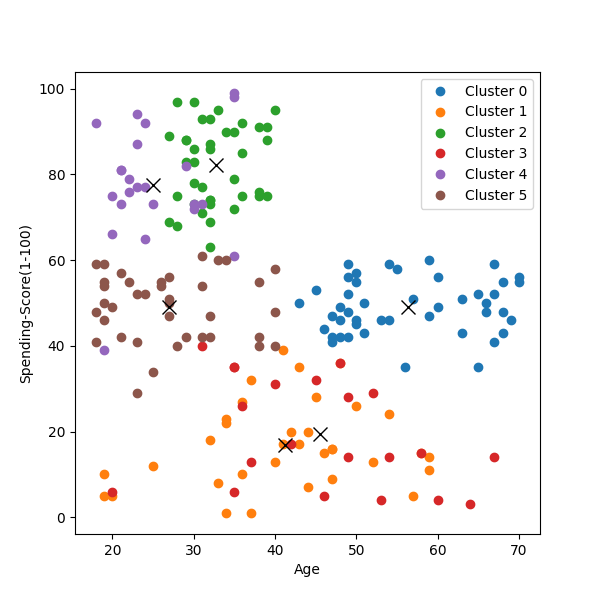
\includegraphics[width=\textwidth]{./Prob4/out/task2_rand14/images/cluster_result_k6_0_2.png}
        \caption{Age vs. Spending Score}
        \label{fig: Age vs. Spending Score k6 rand14 pp}
    \end{minipage}
    \hfill
    \begin{minipage}{0.32\textwidth}
        \centering
        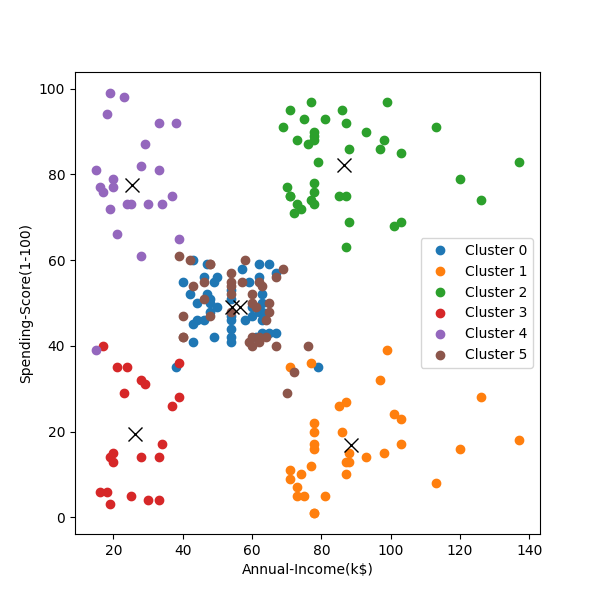
\includegraphics[width=\textwidth]{./Prob4/out/task2_rand14/images/cluster_result_k6_1_2.png}
        \caption{Annual Income vs. Spending Score}
        \label{fig: Annual Income vs. Spending Score k6 rand14 pp}
    \end{minipage}
    \hfill
    \begin{minipage}{0.32\textwidth}
        \centering
        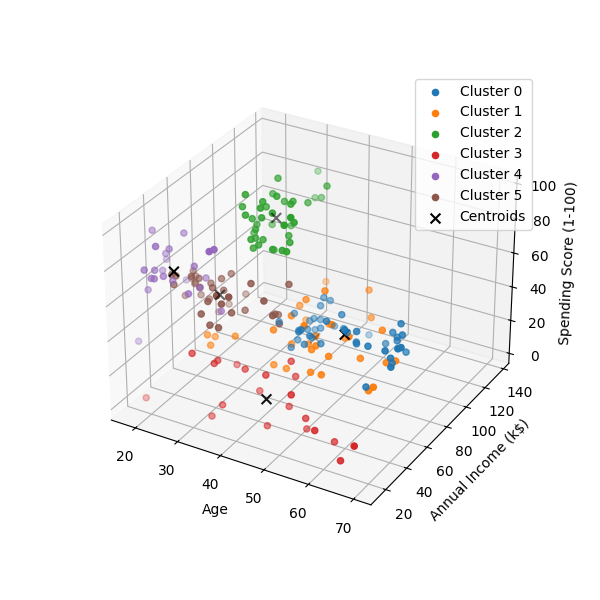
\includegraphics[width=\textwidth]{./Prob4/out/task2_rand14/images/cluster_result_k6_3d.png}
        \caption{3D Visualization}
        \label{fig: 3D Visualization k6 rand14 pp}
    \end{minipage}
    \hfill
    \begin{minipage}{0.32\textwidth}
        \centering
        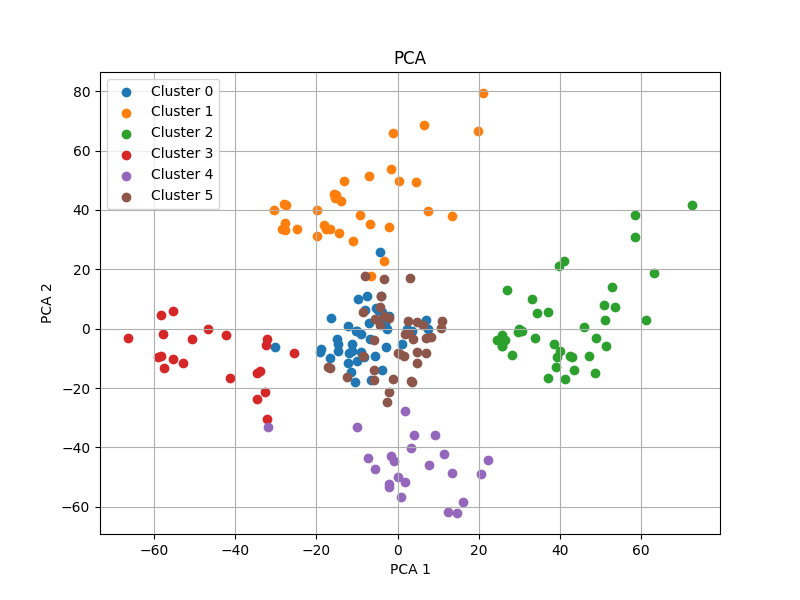
\includegraphics[width=\textwidth]{./Prob4/out/task2_rand14/images/PCA_k6.png}
        \caption{PCA Visualization}
        \label{fig: PCA Visualization k6 rand14 pp}
    \end{minipage}
    \hfill
    \begin{minipage}{0.32\textwidth}
        \centering
        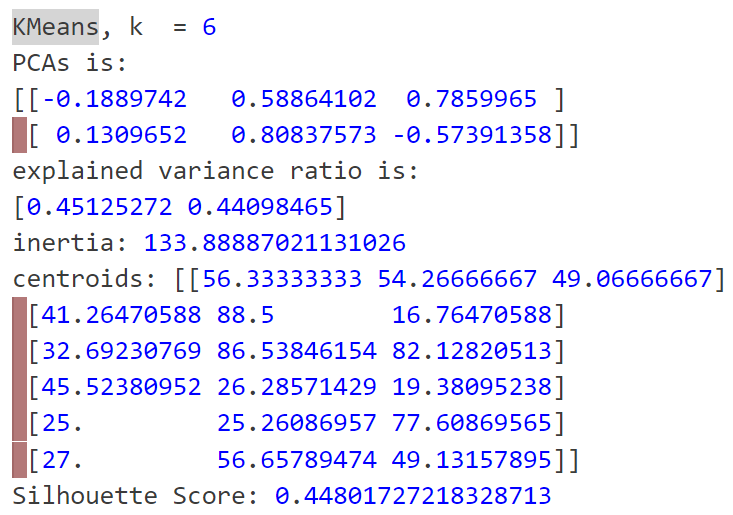
\includegraphics[width=\textwidth]{./Prob4/out/task2_rand14/log_k6.png}
        \caption{Log}
        \label{fig: log_k6.png rand14 pp}
    \end{minipage}
\end{figure}

2.1. 实现聚类评估指标,代码见 {\color{blue}Prob4/utils.py}

图见下

2.2. 对比分析

2.2.1. 以 K = 6,randseed = 14 为例,对比结果差异,可视化图如下:

\begin{figure}[H]
    \centering
    \begin{minipage}{0.32\textwidth}
        \centering
        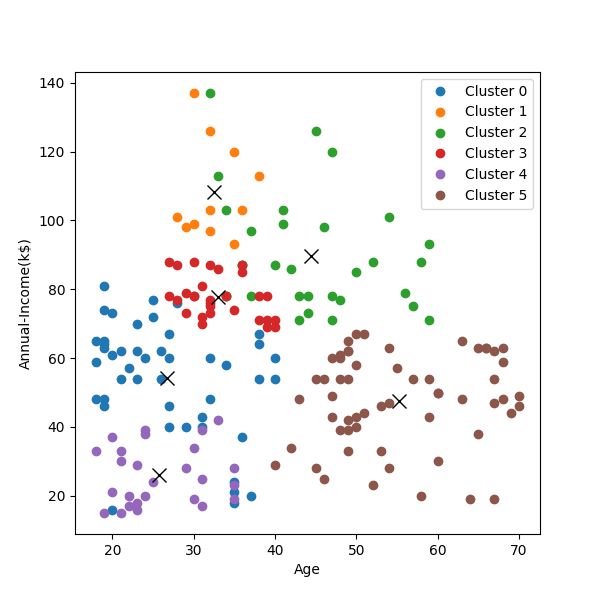
\includegraphics[width=\textwidth]{./Prob4/out/task1_rand14/images/cluster_result_k6_0_1.png}
        \caption{Kmeans: Age vs. Income}
        \label{fig: Age vs. Annual Income k6 com}
    \end{minipage}
    \hfill
    \begin{minipage}{0.32\textwidth}
        \centering
        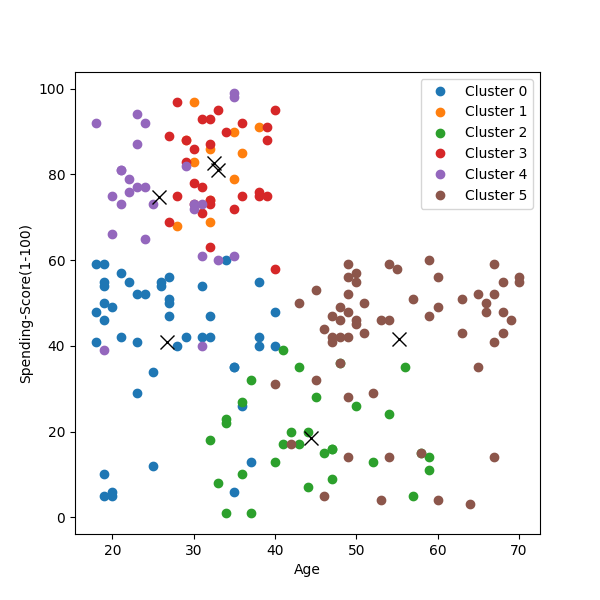
\includegraphics[width=\textwidth]{./Prob4/out/task1_rand14/images/cluster_result_k6_0_2.png}
        \caption{Kmeans: Age vs. Spending}
        \label{fig: Age vs. Spending Score k6 rand14 com}
    \end{minipage}
    \hfill
    \begin{minipage}{0.32\textwidth}
        \centering
        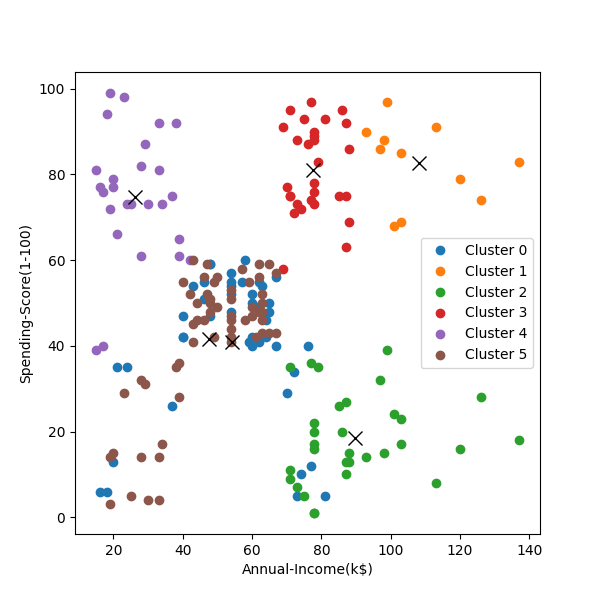
\includegraphics[width=\textwidth]{./Prob4/out/task1_rand14/images/cluster_result_k6_1_2.png}
        \caption{Kmeans: Income vs. Spending}
        \label{fig: Annual Income vs. Spending Score k6 rand14 com}
    \end{minipage}
    \hfill
    \begin{minipage}{0.32\textwidth}
        \centering
        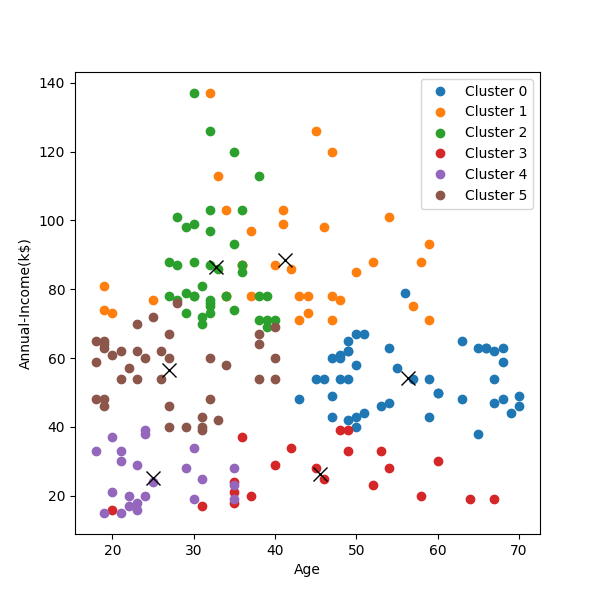
\includegraphics[width=\textwidth]{./Prob4/out/task2_rand14/images/cluster_result_k6_0_1.png}
        \caption{Kmeans++: Age vs. Income}
        \label{fig: Age vs. Annual Income k6 pp com}
    \end{minipage}
    \hfill
    \begin{minipage}{0.32\textwidth}
        \centering
        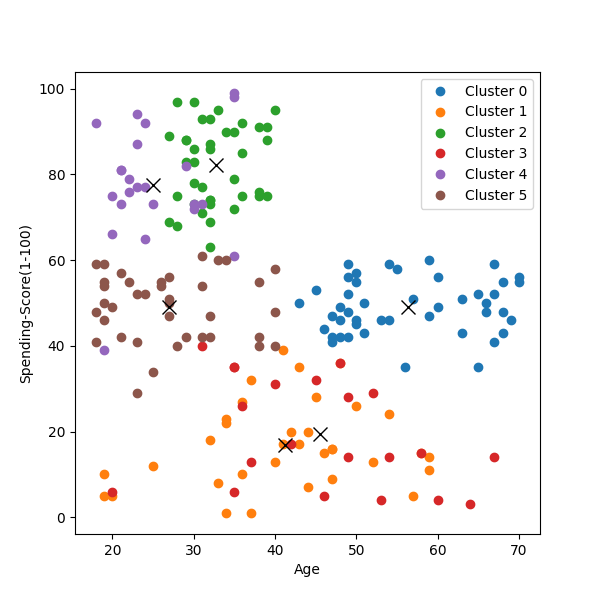
\includegraphics[width=\textwidth]{./Prob4/out/task2_rand14/images/cluster_result_k6_0_2.png}
        \caption{Kmeans++: Age vs. Spending}
        \label{fig: Age vs. Spending Score k6 rand14 pp com}
    \end{minipage}
    \hfill
    \begin{minipage}{0.32\textwidth}
        \centering
        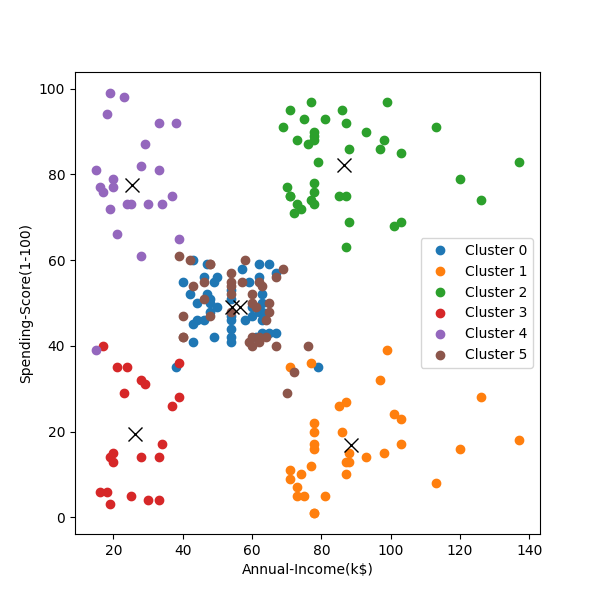
\includegraphics[width=\textwidth]{./Prob4/out/task2_rand14/images/cluster_result_k6_1_2.png}
        \caption{Kmeans++: Income vs. Spending}
        \label{fig: Annual Income vs. Spending Score k6 rand14 pp com}
    \end{minipage}
    \hfill
\end{figure}

从图中可以看出,
随机初始化细分了高收入高积分人群,即图\ref{fig: Age vs. Annual Income k6 com}-图\ref{fig: Annual Income vs. Spending Score k6 rand14 com}中的Cluster1和Cluster3,
但是对于中低收入中低积分的人群,即图\ref{fig: Age vs. Annual Income k6 com}-图\ref{fig: Annual Income vs. Spending Score k6 rand14 com}中的Cluster 0和Cluster 5的分类明显不当;
而Kmeans++,则将中低收入中低积分的人群细分为图\ref{fig: Age vs. Annual Income k6 pp com}-图\ref{fig: Annual Income vs. Spending Score k6 rand14 pp com}中的Cluster 0, Cluster 3 和 Cluster5,
并把一部分中等收入群体分类到中高收入人群(图\ref{fig: Age vs. Annual Income k6 pp com}-图\ref{fig: Annual Income vs. Spending Score k6 rand14 pp com}中的Cluster 1)中,分类更加合理。

\begin{figure}[H]
    \centering
    \begin{minipage}{0.45\textwidth}
        \centering
        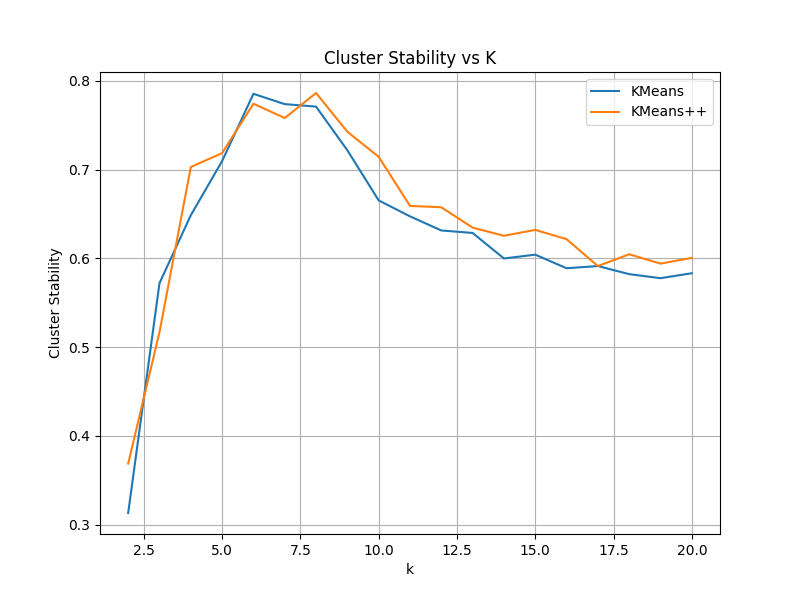
\includegraphics[width=\textwidth]{./Prob4/out/task_2_2/stabilities_k20.png}
        \caption{Stability vs. K}
        \label{fig: Kmeans vs. Kmeans++ Stability 50rounds}
    \end{minipage}
    \hfill
    \begin{minipage}{0.45\textwidth}
        \centering
        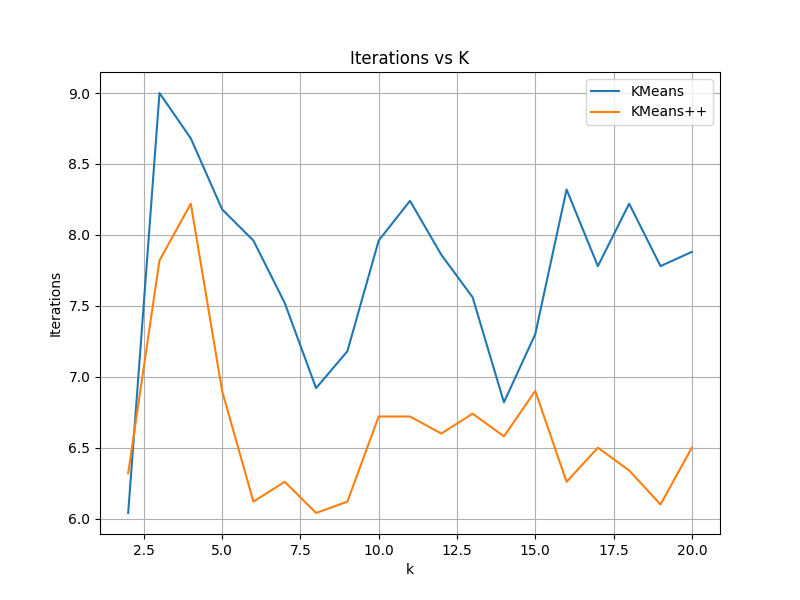
\includegraphics[width=\textwidth]{./Prob4/out/task_2_2/iters_k20.png}
        \caption{iters vs. K}
        \label{fig: Kmeans vs. Kmeans++ iters 50rounds}
    \end{minipage}
    \hfill
\end{figure}

2.2.2. 比较两种方法的稳定性:

我们采取了50轮的随机实验(不固定随机种子),计算了两种初始化方法的稳定性,并取平均值,见图\ref{fig: Kmeans vs. Kmeans++ Stability 50rounds}。可见,平均来看两者稳定性相差不大。

2.2.3. 分析初始化对收敛速度的影响:

我们采取了50轮的随机实验(不固定随机种子),计算了两种初始化方法的迭代轮数,并取平均值,见图\ref{fig: Kmeans vs. Kmeans++ iters 50rounds}。可见,Kmeans++方法的收敛速度更快。

\vspace{3em}

3. 在实际业务中,不同特征的重要性可能不同,且某些客户群可能需要大小相近。请实现带权重和大小约束的改进版本:
\begin{itemize}
    \item 实现带约束的聚类算法,需要支持特征加权和簇大小约束(4 points)
    \item 在以下两个场景下重新进行实验:收入特征权重加倍,限制每个客户群至少包含20\%的客户, 绘制聚类结果(6 points)
\end{itemize}
\begin{lstlisting}[language=Python, caption=带约束的聚类算法部分实现]
class ConstrainedKMeans(KMeansPlusPlus):
    def __init__(self, n_clusters=3, max_iters=100, weights=None, size_constraints=None):
        """
        参数:
            weights: 特征权重向量
            size_constraints: 每个簇的最小和最大样本数量限制
        """
        super().__init__(n_clusters, max_iters)
        self.weights = weights
        self.size_constraints = size_constraints
        
    def _weighted_distance(self, X, centroids):
        """计算加权欧氏距离"""
        pass
        
    def _reassign_clusters(self, X, labels, distances):
        """在满足大小约束的情况下重新分配样本到簇"""
        pass
\end{lstlisting}


\textbf{\large 解:}

\vspace{3em}


\end{document}
